\subsection{Sequence Diagram}

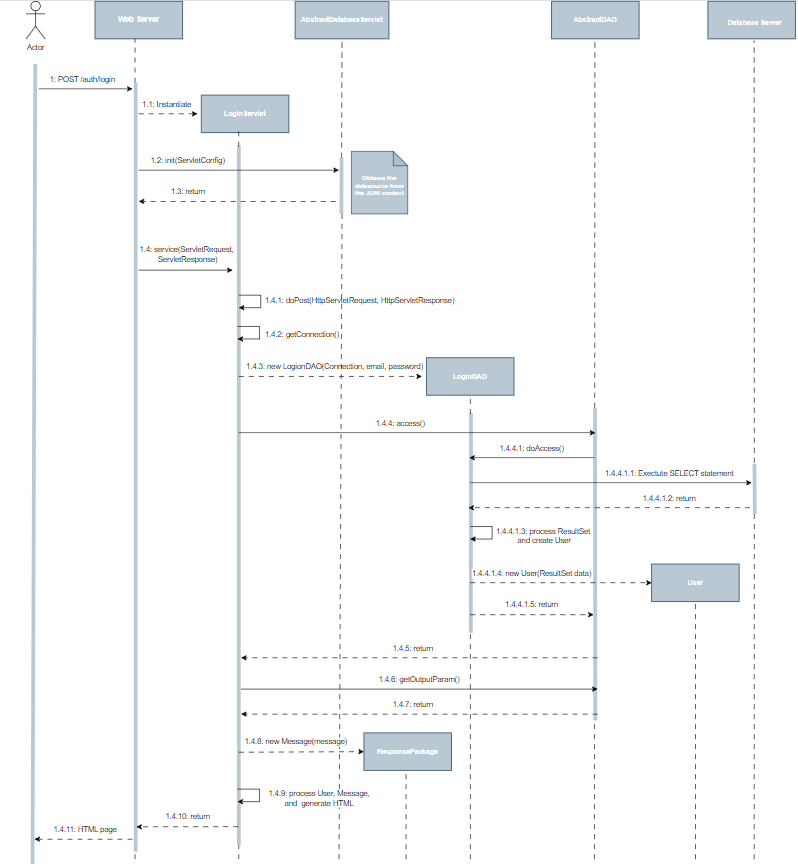
\includegraphics[scale = 0.8]{sections/BLL/sequenceDiagram.png}

\textbf{DA MODIFICARE:}
Here is reported the sequence diagram for the operation about the insert of a simple user. The user
executes a POST request to the web server. The web server instantiates the UserServlet, get the
information about the datasource from the init method of the AbstractDatabaseServlet. After that it
calls the doPost method of the UserServlet, passing the HttpServletRequest and the HTTP Servlet
response. The UserServlet analyzes the request and recognizes that it is an insert operation, thus it
creates an object User with the request parameters. At last, with the using of the insertNewUser
method of the UserDAO class, the servlet inserts the User in the database. After that, the UserServlet
replies to the web server with the methods setStatus and getWriter that notify if everything goes well
or not.